\documentclass[10pt,a4paper]{article}
\usepackage[a4paper, total={6in, 8in}]{geometry}
\usepackage{graphicx}
\usepackage{scrlayer-scrpage}
\clearpairofpagestyles


\begin{document}
\chead{Stefanie North (51803598) | Stefan Rietzinger (11910536) | Theo Dorfner (11909414)}
\cfoot{\pagemark}

\section{Task: Questions (3 points)}

\subsection{Comparison of 1D and 2D decomposition}

\textbf{Describe the advantages/disadvantages of a two-dimensional decomposition (compared to a one-dimensional decomposition).}\\

At first glance, it seems to be an advantage of the 1D decomposition that only two neighbours have to be sent to, which 
means less work than sending to all four neighbours as in the 2D case. However, if you look at the actual data that is going 
to be sent and the time it takes, the 2D decomposition hase actually an advantage. A good parameter is the speedup, 
which is calculated by dividing the runtime $T_s$ by the parallel runtime $T_p$. $S = \frac{T_s}{T_p}$, this indicates 
how much the runtime changes by including more processes. Overall, it can be said that the scaling behaviour 
between 1D decomposition and 2D decomposition is significantly different, as the intersection of the 2D subdomains is 
smaller than in the 1D case. However, this does not have a significant effect on the speed-up when the number of CPU 
cores is small, but it does when the number is large. \\


To illustrate this, we can consider an example: We take a domain with a resolution of 250 and calculate 100 time steps. 
We describe $t_s$ as the time needed to calculate one iteration for one node and $t_p$ as the time needed to communicate 
with other cells and assume that both take one time unit. \\
\\
\begin{center}
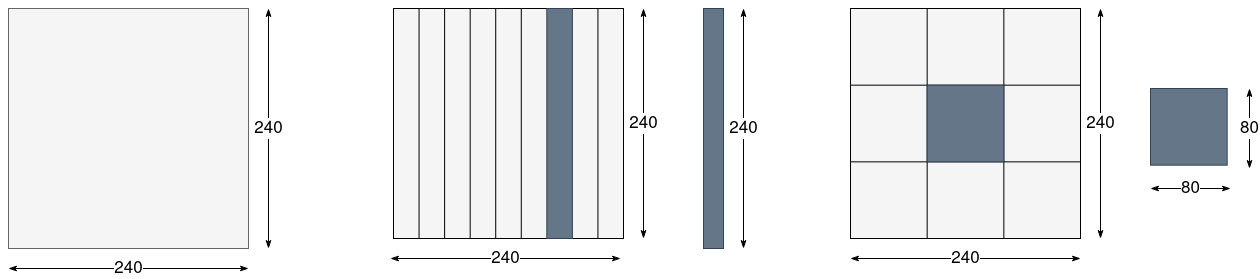
\includegraphics[width=14.5cm]{images/Task.png}
\end{center}

In the figure above, an area with a resolution of 240 is shown, the entire domain can be seen on the left. If a 1D 
decomposition were chosen, the sub-areas would look like the blue rectangle in the middle, with the cutting surface 
to be communicated being 2x240 = 480. The 2D decomposition is shown on the right. Here the edge of the subarea is 
4x80 = 320. \\

\begin{table}[h]
    \centering
    \begin{tabular}{l|l|l}
    \textbf{MIP processes} & \textbf{1D Speedup} & \textbf{2D Speedup} \\ \hline
    5                      & 4.8             & 4.97            \\ \hline
    25                     & 20.83           & 24.38           \\ \hline
    125                    & 62.5            & 110.96          \\ \hline
    250                    & 83.33           & 199.53          \\
    \end{tabular}
\end{table}

It can be seen from the table that the speedup scales much better with resolution in 2D decomposition, as the 
intersection of the domains remains the same in 1D at any resolution, but becomes smaller in 2D as the resolution 
increases. \\

Reference : https://alexander.vondrous.de/?p=7

\newpage
\subsection{Effect of decomposition on numercal solution}

\textbf{Discuss if the decomposition of the domain changes the order of computations performed during a single Jacobi 
iteration -  i.e., if you expect a numerically identical result after each iteration, or not.} \\

Since the decomposition now divides the area into smaller sub-areas, but does not change the actual values. Also, 
in our code, the boundaries of the subdomains are updated with the neighbouring values at each iteration. We expect 
that the result after each iteration will not be numerically different from the calculation without subdomains, to 
machine precision. If the ghost values were updated less frequently, we expect the error to increase. \\

\subsection{Depth of ghost layer}

\textbf{A generalization of the ghost layer approach would be to set the width of the ghost 
layer that is exchanged as a parameter W of the decomposition. This allows to perform W independent 
iterations before a communication of the ghost layers has to happen. Comment in which situation 
(w.r.t the available bandwidth or latency between MPI-processes) multiple independent iterations are 
potentially advantageous.} \\


In the approach of a ghost layer with a depth of one, one would have to update the boundaries of the sub-areas at 
each step and therefore send many messages with a small size. This is a large communication overhead. Generalising 
this approach, as described in the question, to a ghost layer with a width of W fixes this, but the number of ghost 
layers also corresponds to the accuracy of the numerical methods.\\

The idea behind this generalisation of the ghost layers is the increase in message volume with each update and 
correspondingly less frequent updating in general. This means with W = 6, the ghost layers only need to be updated 
once every five time steps, with six layers being exchanged at once. So with less frequent updates, smaller messages 
are combined into larger messages, allowing for higher communication bandwidth and lower communication latency. \\ 

This can be advantageous if the available bandwidth allows it. Since we are working with the IUE cluster, a bandwidth 
of 10Gbit/s is available. Even when reducing latency is the main goal, changing the width of the ghost layers can be 
a good approach. One disadvantage of a larger W is that this method requires more memory and computation than the 
traditional method, but this is a small difference compared to the total memory required. \\ 
 
Reference: DOI: 10.1109/SC.2001.10042 \\

\newpage
\subsection{Exchange with diagional neighbors}

\textbf{Assume a ghost layer with width W=1 (this is what you will later implement) 
and discuss if a data exchange between parts of the domain which are "diagonal neighbors" is 
required assuming a "5-point star-shaped stencil".} \\

Since we work with a "5-point star template", the diagonal elements are never needed for an iteration. Only the 
direct neighbours in the direction of north, south, west, east are needed. Furthermore, if the communication with 
the ghost layers involves all elements in a row/column, as implied in the task description and in the figure below, 
it is possible to exchange data with the "diagonal neighbours" in two steps as well. This is illustrated in the 
following figure. \\


\begin{center}
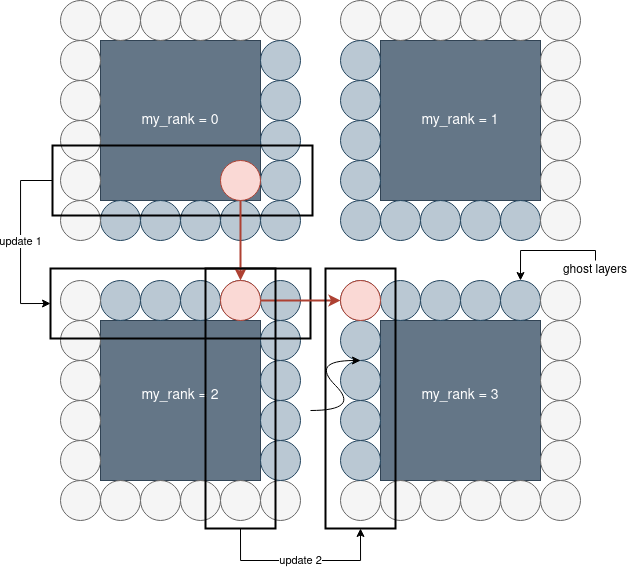
\includegraphics[width=7cm]{images/Diagonal.png}
\end{center}

\subsection{IUE-cluster}
\textbf{How big is the sum of all L2 caches for 2 nodes of the IUE-cluster }\\


Looking at the statistics of the IUE cluster, there are two types of computer nodes available, 10x normal 
computer nodes and 2x fat computer nodes. Both types are equipped with 2x INTEL Xeon Gold 6248, 2.5GHz, 20C/40T, 
as described on the official website. [1] So each processor has an L2 cache of 16MB [2], giving a total of 64MB 
for 2 nodes and 2 INTEL. \\


Reference:
\begin{enumerate}
    \item [1] https://www.iue.tuwien.ac.at/research/computing-infrastructure/
    \item [2] https://www.cpubenchmark.net
\end{enumerate}



\newpage
\section{Task: One-Dimensional Decomposition (4 points)}

As a first approach, an explicit definition of the matrix A was chosen, which also gave us the right results 
and a good runtime. However, we also encountered limitations in our attempt to run with a higher resolution, 
since the size of the matrix increases extremely with the resolution. This requires a very large memory, which we 
had neither on our local computers nor on the cluster. Therefore, we had to use a new approach. To reduce the memory 
we chose and implemented "Coordinate Format" (COO), which was a good option because A is a sparse matrix. Now we 
had no more memory problems but the runtime was extremely slowed down. This was not a satisfactory solution 
either. The third and final version was to exploit the regularity and structure of A and to no longer 
define the matrix explicitly. In the Jacobi steps, if/else if loops are used to explicitly determine how 
the "matrix-vector" multiplication must proceed. That is, which elements of u(x) must be multiplied by which 
pre-factor. This allowed us to have a fast and memory-efficient solution. 

\subsection{Implementation}

%Stefan

After creating of an MPI environment and determining the rank of the processes, a one-dimensional "MPI Cart" was created. The next step was to assign the dimensions for the individual "blocks" of the MPI Cart. To do this, a function was created that divided the resolution by the number of processes and floored the result.
Then the modulo of the resolution by the number of processes was determined and added to each process individually.
For illustration: With a dimension of unknowns of 9 and a process number of 4 the output would be 3,2,2,2.
This function was now used to construct the right hand side b. For this all X and Y values 
of the unknowns in the respective "block" were determined, the function was evaluated at this point and appended to b. If the Y-values are in the 
lowest row (Y == (1-h)) the boundary condition is added.
\\ 

%Theo
In order to be able to run the iterations we must first retrieve the addresses of the neighbours, which 
can be done using MPI Cart Shift. Even for the 1D version we could technically use the 2D code, as 
missing  neighbours just produce an address rank of -2, which terminates the respective communication 
when used as a target rank.\\

During each iteration we start of by calculating the outgoing ghost-layer values from the results of the
previous iteration. Then we initialize non-blocking receives to all neighbours, followed by blocking sends 
to all neighbours. Afterwards each process waits for the non-blocking receives to terminate, which allows 
it to then write the received ghostValues into one large ghostVector of the same size as the linear system.
The jacobi iteration then cacluates the new solution vector, using the ghostVector on the right hand side. 
In order to avoid large vectors for high resolution (and because it produced errors when originally running) we don't implement a Matrix A anymore, but rather do the generation of the matrix elements directly when using them. Each iteration is timed.
After finishing the iterations, each process calculates the mean runtime per iteration and prepars the 
solution, as well as the right hand side, for residual and error calculation. \\

%Steffi
After the final results have been computed, the residuals and the errors are calculated for each rank. To 
simplify the collection of all results, four values are stored per rank. The maximum residual, the 
maximum error and the squared l2 norm of the residual and the error. With MPI Reduce, the elements are then 
collected at rank 0 and either added directly in the case of the l2 norm or the maximum is found to calculate
infinite norm. The average runtime per rank is also added up and divided by the total number of processes 
to get the total time. All results are then output.

\newpage
\subsection{Analysis}

In this section the parallel speedup and parallel efficiency are calculated and analysed. Bei der Analyser 
des Parrallel speed up wurden der absolute und der relative speed up berechnet. 

\begin{center}
    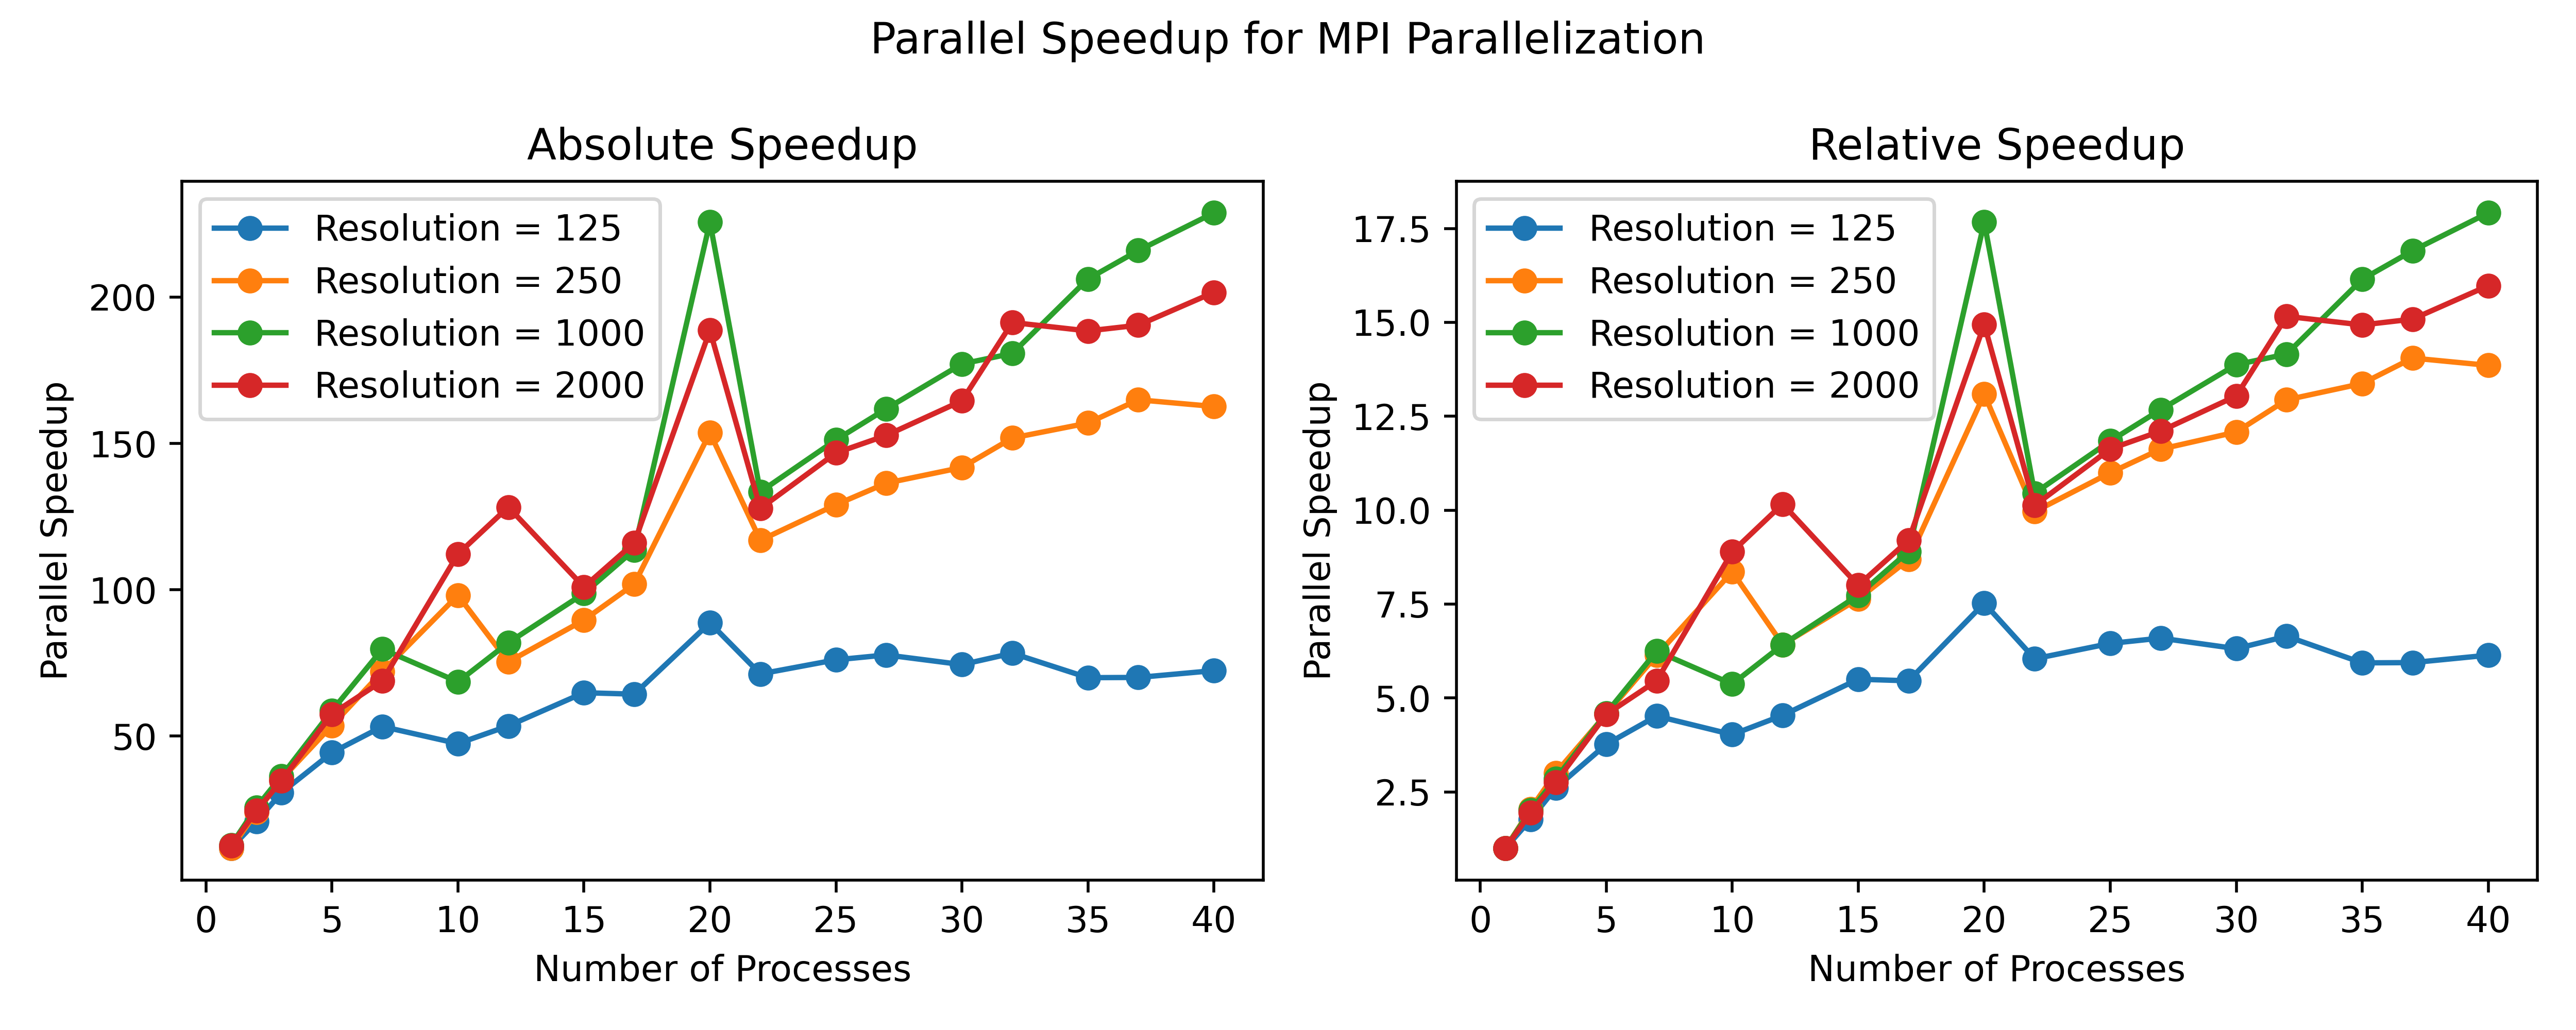
\includegraphics[width=15cm]{analysis/parallelSpeedup_1.png}
\end{center}

The absolute speedup was compared with the serialtime of the provided Jacobisolver. The relative speedup 
is relative to our solver when running with one process. In both plots the respective speedup is shown with 
different resolutions with 0-40 MPI processes. All in all it can be said that with more processes being 
utitlized the computaion get faster, as expected. \\

The absolute speedup is linear for all resolutions in the beginning, then as expected the messurements 
diverge from the linear behavior. This divergent behavior is dependent on the chosen resolution as here is 
a certain limit above which each process has so little to do that adding a process does not make such a 
big difference in the computing effort per process. Accordingly, it is clear that the flattening happens 
later at a higher resolution. This is exactly what we can observe in our implementation. The same behavior 
can be seen in the plot of the realtive speedup. \\



Auffalend ist der Peak bei 20 Processes da dieser bei jeder Auflösung zusehen ist. 
Anscheinend ist die Wahl von 20 Processes besonders gut geeingent. Dies ist auch 
erwartbar da die Computernodes die wir am Cluster verwenden pro node 2 INTEL Xeon 
Gold 6248, 2.5GHz, 20C/40T processors besitzt. Bei einer Wahl von 20 werden also 
genau alle Cores von einer Intel verwendet. 


\begin{center}
    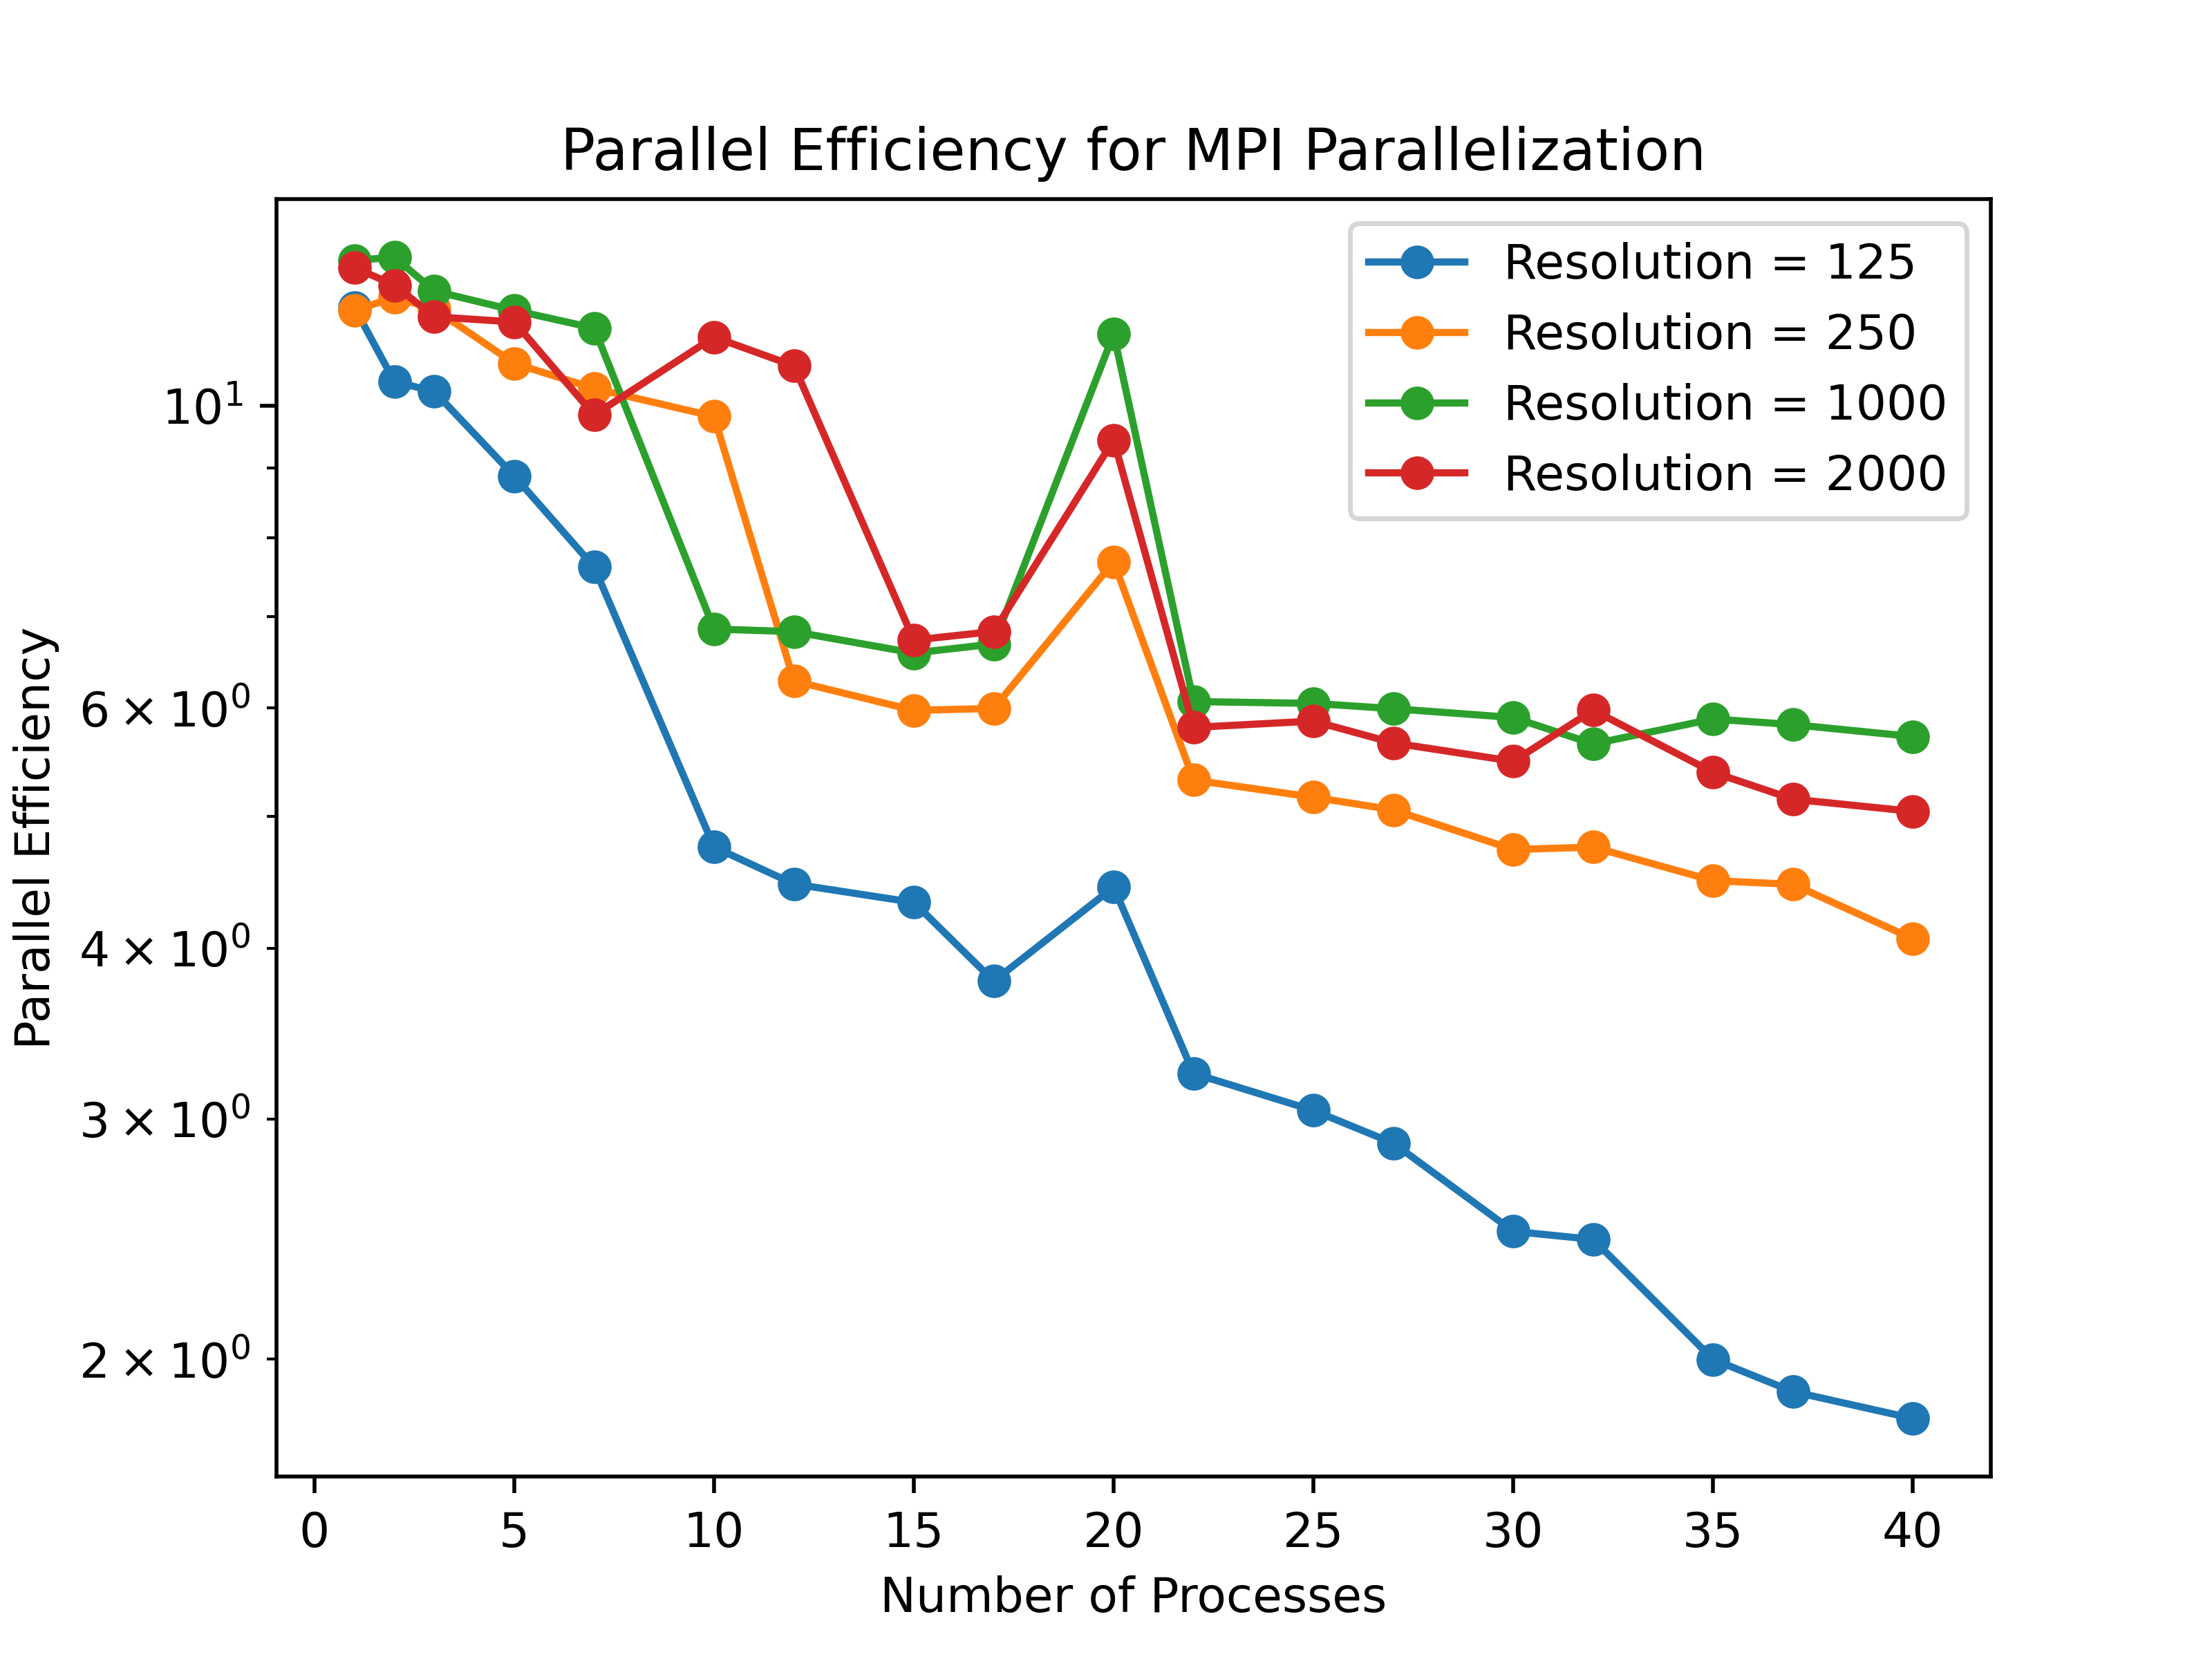
\includegraphics[width=10cm]{analysis/parallelEfficiency.png}
\end{center}

In the third graph you can see the parallel efficiency (relative to the provided code). 
The parallel efficiency obtained behaves as expected and decreases as the number of 
processors increases. The slope depends on the resolution and decreases with increasing 
resolution. Again, a peak is seen at 20 processes for the same reason. It is also 
interesting that there is a relatively large difference between res:125 and the rest 
of the resolutions.

\section{Task: Two-Dimensional Decomposition (3 points)}

The code for doing the iterations in the case of 2D barely changed from the case of 1D. Theoretically it 
should be possible to simply use the 2D code for 1D executions. The reason for this is, that MPI just 
gives back a non-communicator (rank = -2) for non existing neighbours.
\\
The most important difference compared to 1D decomposition is that the "blocks" no longer have the same
have the same width in X-direction. However, the X and Y dimensions of the "blocks" are now 
determined using a similar function as in the 1D decomposition. The calculation of the right 
side of the equation system was determined equivalent to the 1D case.


\end{document}
